
\documentclass[border=10pt]{standalone}
\usepackage{pgfplots}
\pgfplotsset{compat=1.18}
\usepgfplotslibrary{colormaps}
\begin{document}
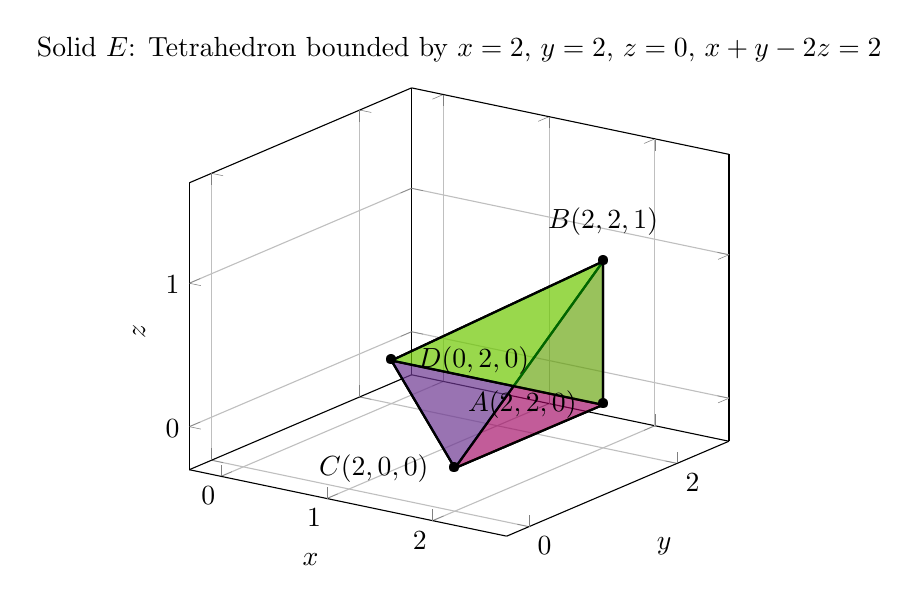
\begin{tikzpicture}
\begin{axis}[
    title={Solid $E$: Tetrahedron bounded by $x=2$, $y=2$, $z=0$, $x+y-2z=2$},
    xlabel={$x$}, ylabel={$y$}, zlabel={$z$},
    xmin=-0.3, xmax=2.7,
    ymin=-0.3, ymax=2.7,
    zmin=-0.3, zmax=1.7,
    view={35}{22},
    grid=major,
    colormap={bluemap}{
        color=(blue) color=(white)
    },
]

% Slanted face (x+y-2z=2): vertices (2,0,0), (0,2,0), (2,2,1)
\addplot3[fill=orange, fill opacity=0.5, draw=black, thick] coordinates {
    (2,0,0) (0,2,0) (2,2,1)
} -- cycle;

% Bottom face z=0: (2,0,0), (0,2,0), (2,2,0)
\addplot3[fill=blue, fill opacity=0.4, draw=black, thick] coordinates {
    (2,0,0) (0,2,0) (2,2,0)
} -- cycle;

% Right face x=2: (2,0,0), (2,2,0), (2,2,1)
\addplot3[fill=red, fill opacity=0.4, draw=black, thick] coordinates {
    (2,0,0) (2,2,0) (2,2,1)
} -- cycle;

% Front face y=2: (0,2,0), (2,2,0), (2,2,1)
\addplot3[fill=green, fill opacity=0.4, draw=black, thick] coordinates {
    (0,2,0) (2,2,0) (2,2,1)
} -- cycle;

% Vertex labels
\node[label={180:{$A(2,2,0)$}}] at (axis cs:2,2,0) {\textbullet};
\node[label={90:{$B(2,2,1)$}}] at (axis cs:2,2,1) {\textbullet};
\node[label={180:{$C(2,0,0)$}}] at (axis cs:2,0,0) {\textbullet};
\node[label={0:{$D(0,2,0)$}}] at (axis cs:0,2,0) {\textbullet};

\end{axis}
\end{tikzpicture}
\end{document}
